
\chapter{Deployment}
	The analysis results are targeted at decision-makers such as financial analysts and strategists. The clustering results can be part of a in-depth financial analysis, and provide a very broad overview on spending.
	
	The questions this overview should answer are:
	\begin{enumerate}
		\item Which spending categories exist?
		\item How does the spending divide onto the categories?
		\item Which magnitude exists between the different amounts spent?
		\item Which vendors are connected to the largest payments?
		\item Which geographical locations are related to the largest payments?
		\item How are the expenses distributed over all locations?
	\end{enumerate}
	
	The results of an analysis are often summarized using a business intelligence visualization tool. In this case, the analysis is visualized using Tableau.
	
	\begin{sidewaysfigure}
			\centering
		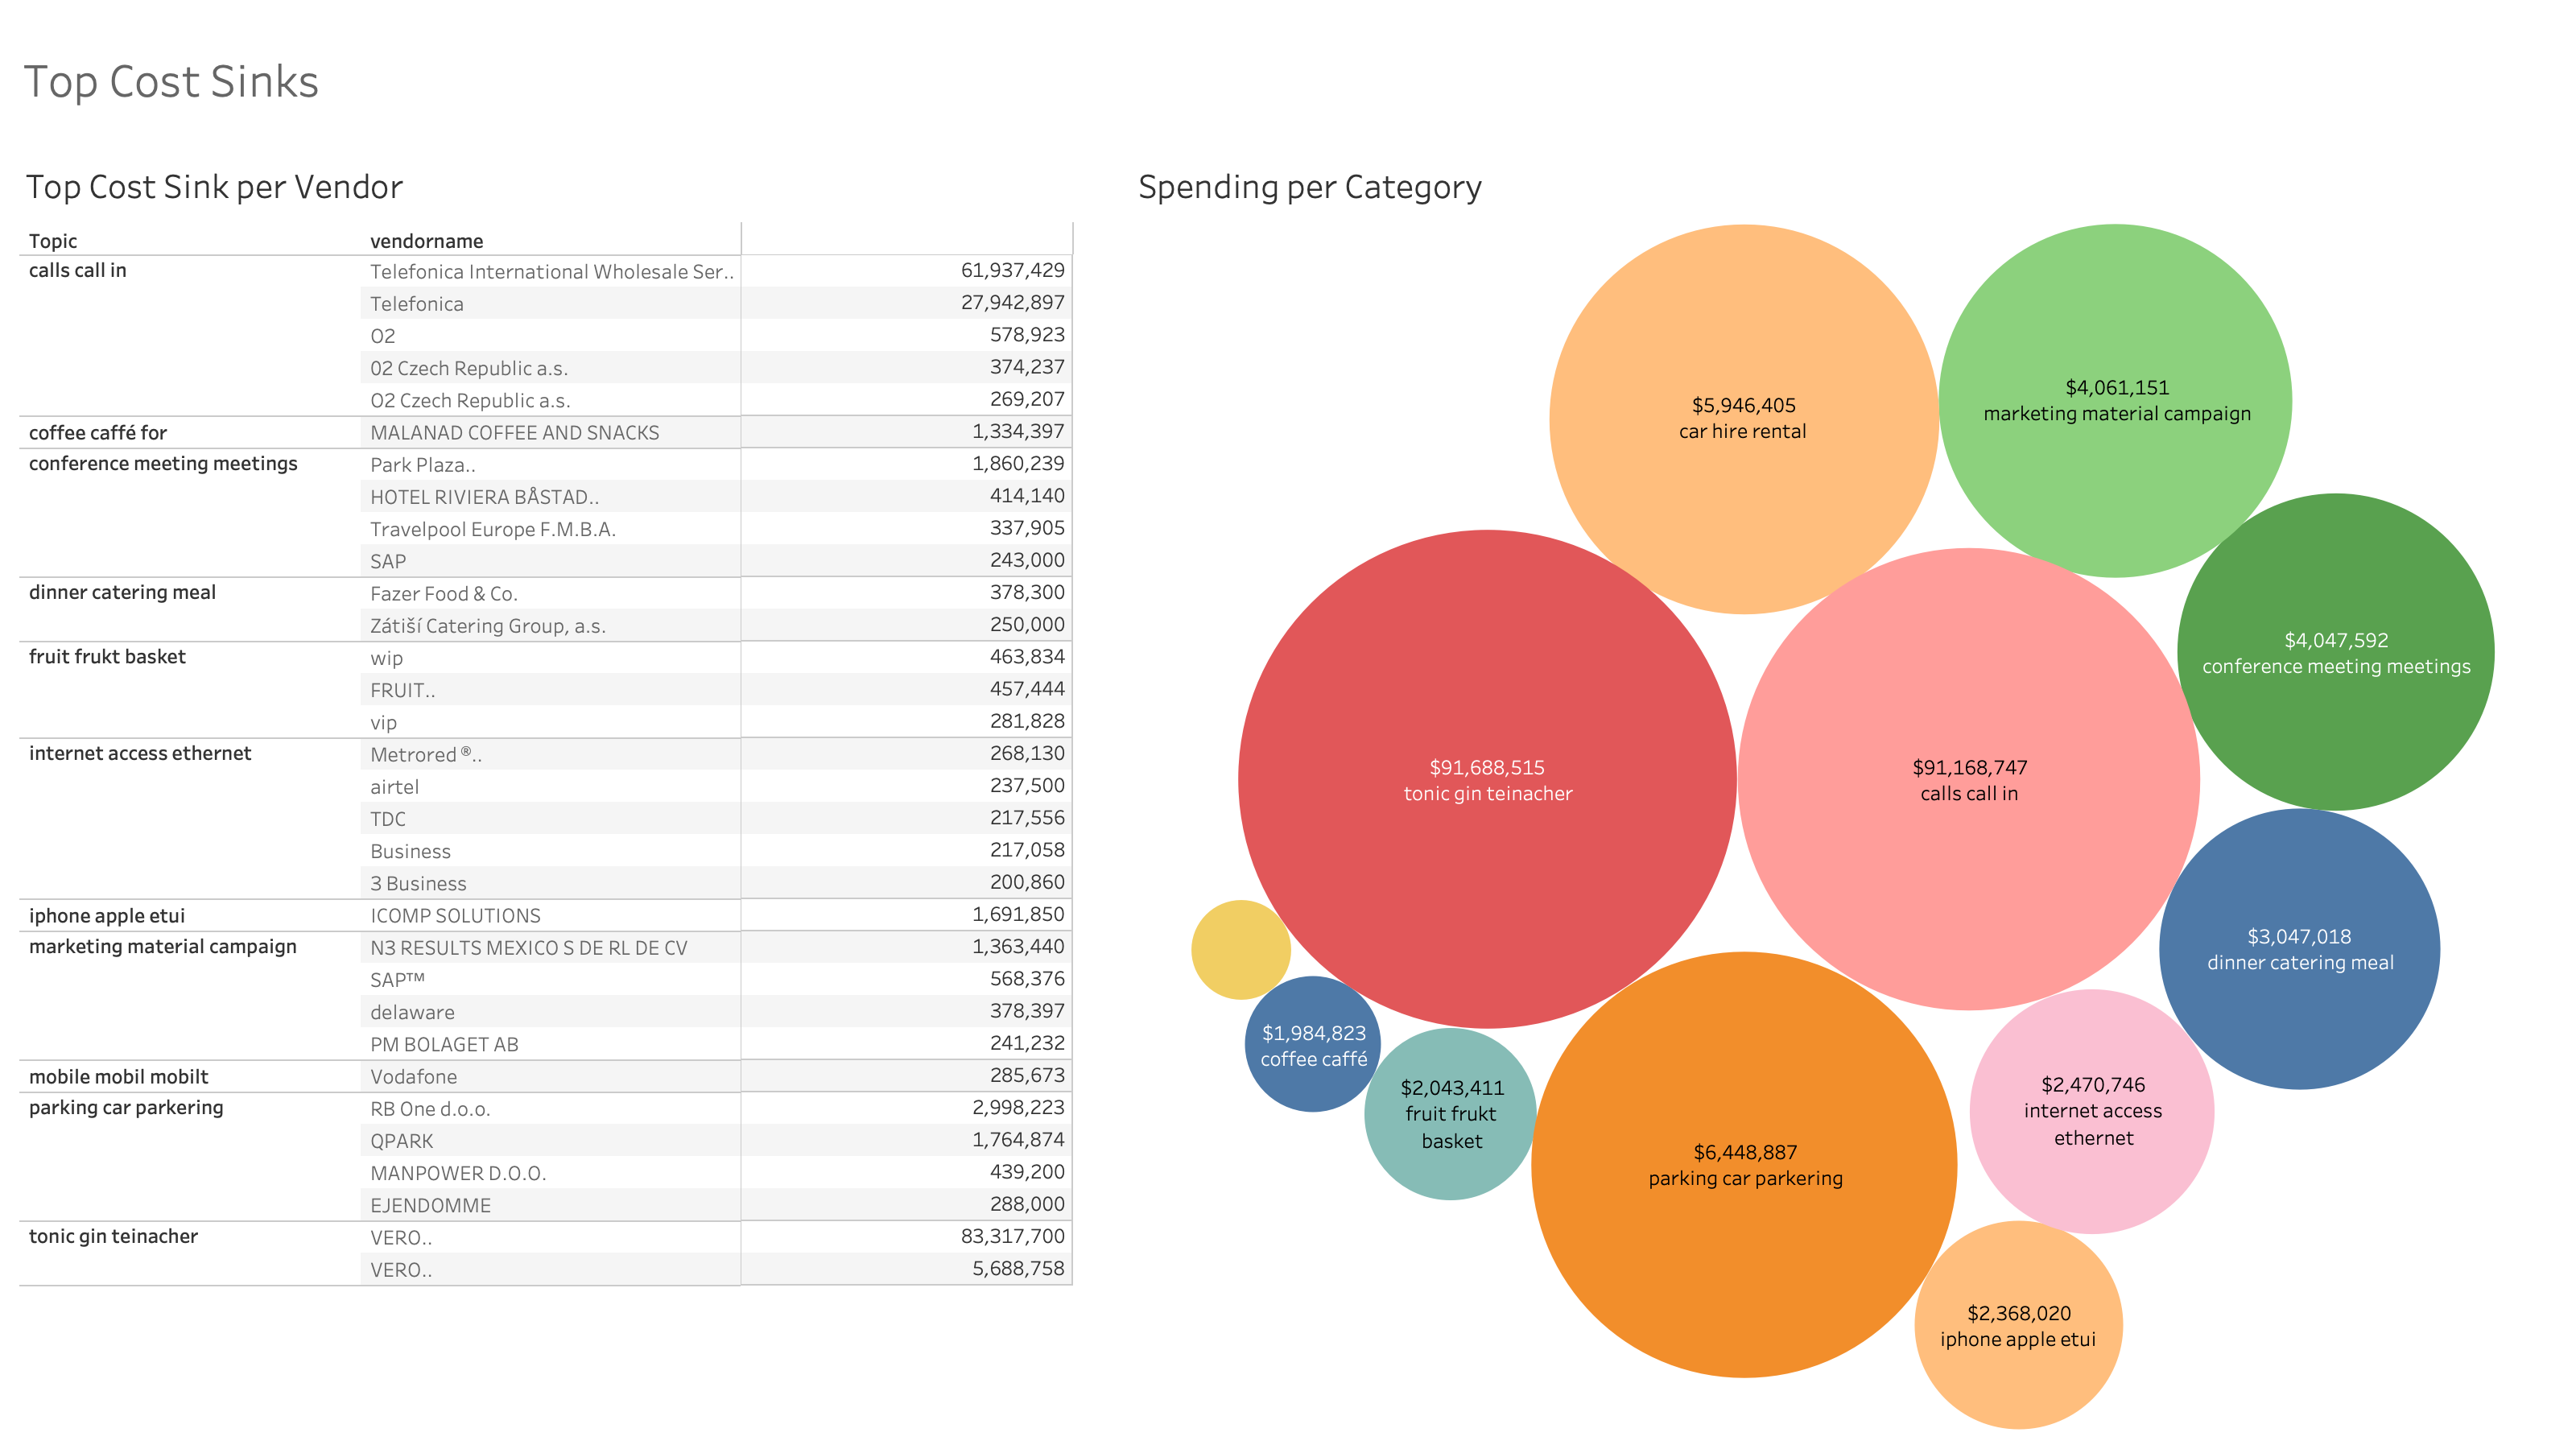
\includegraphics[
		width=\linewidth]{Bilder/deployment/bubble.png}
		\caption{Tableau Dashboard: Overview on the largest Spending Categories}
		\label{fig:dashboard-bubble}
	\end{sidewaysfigure}


\begin{sidewaysfigure}[h!]
	\centering
	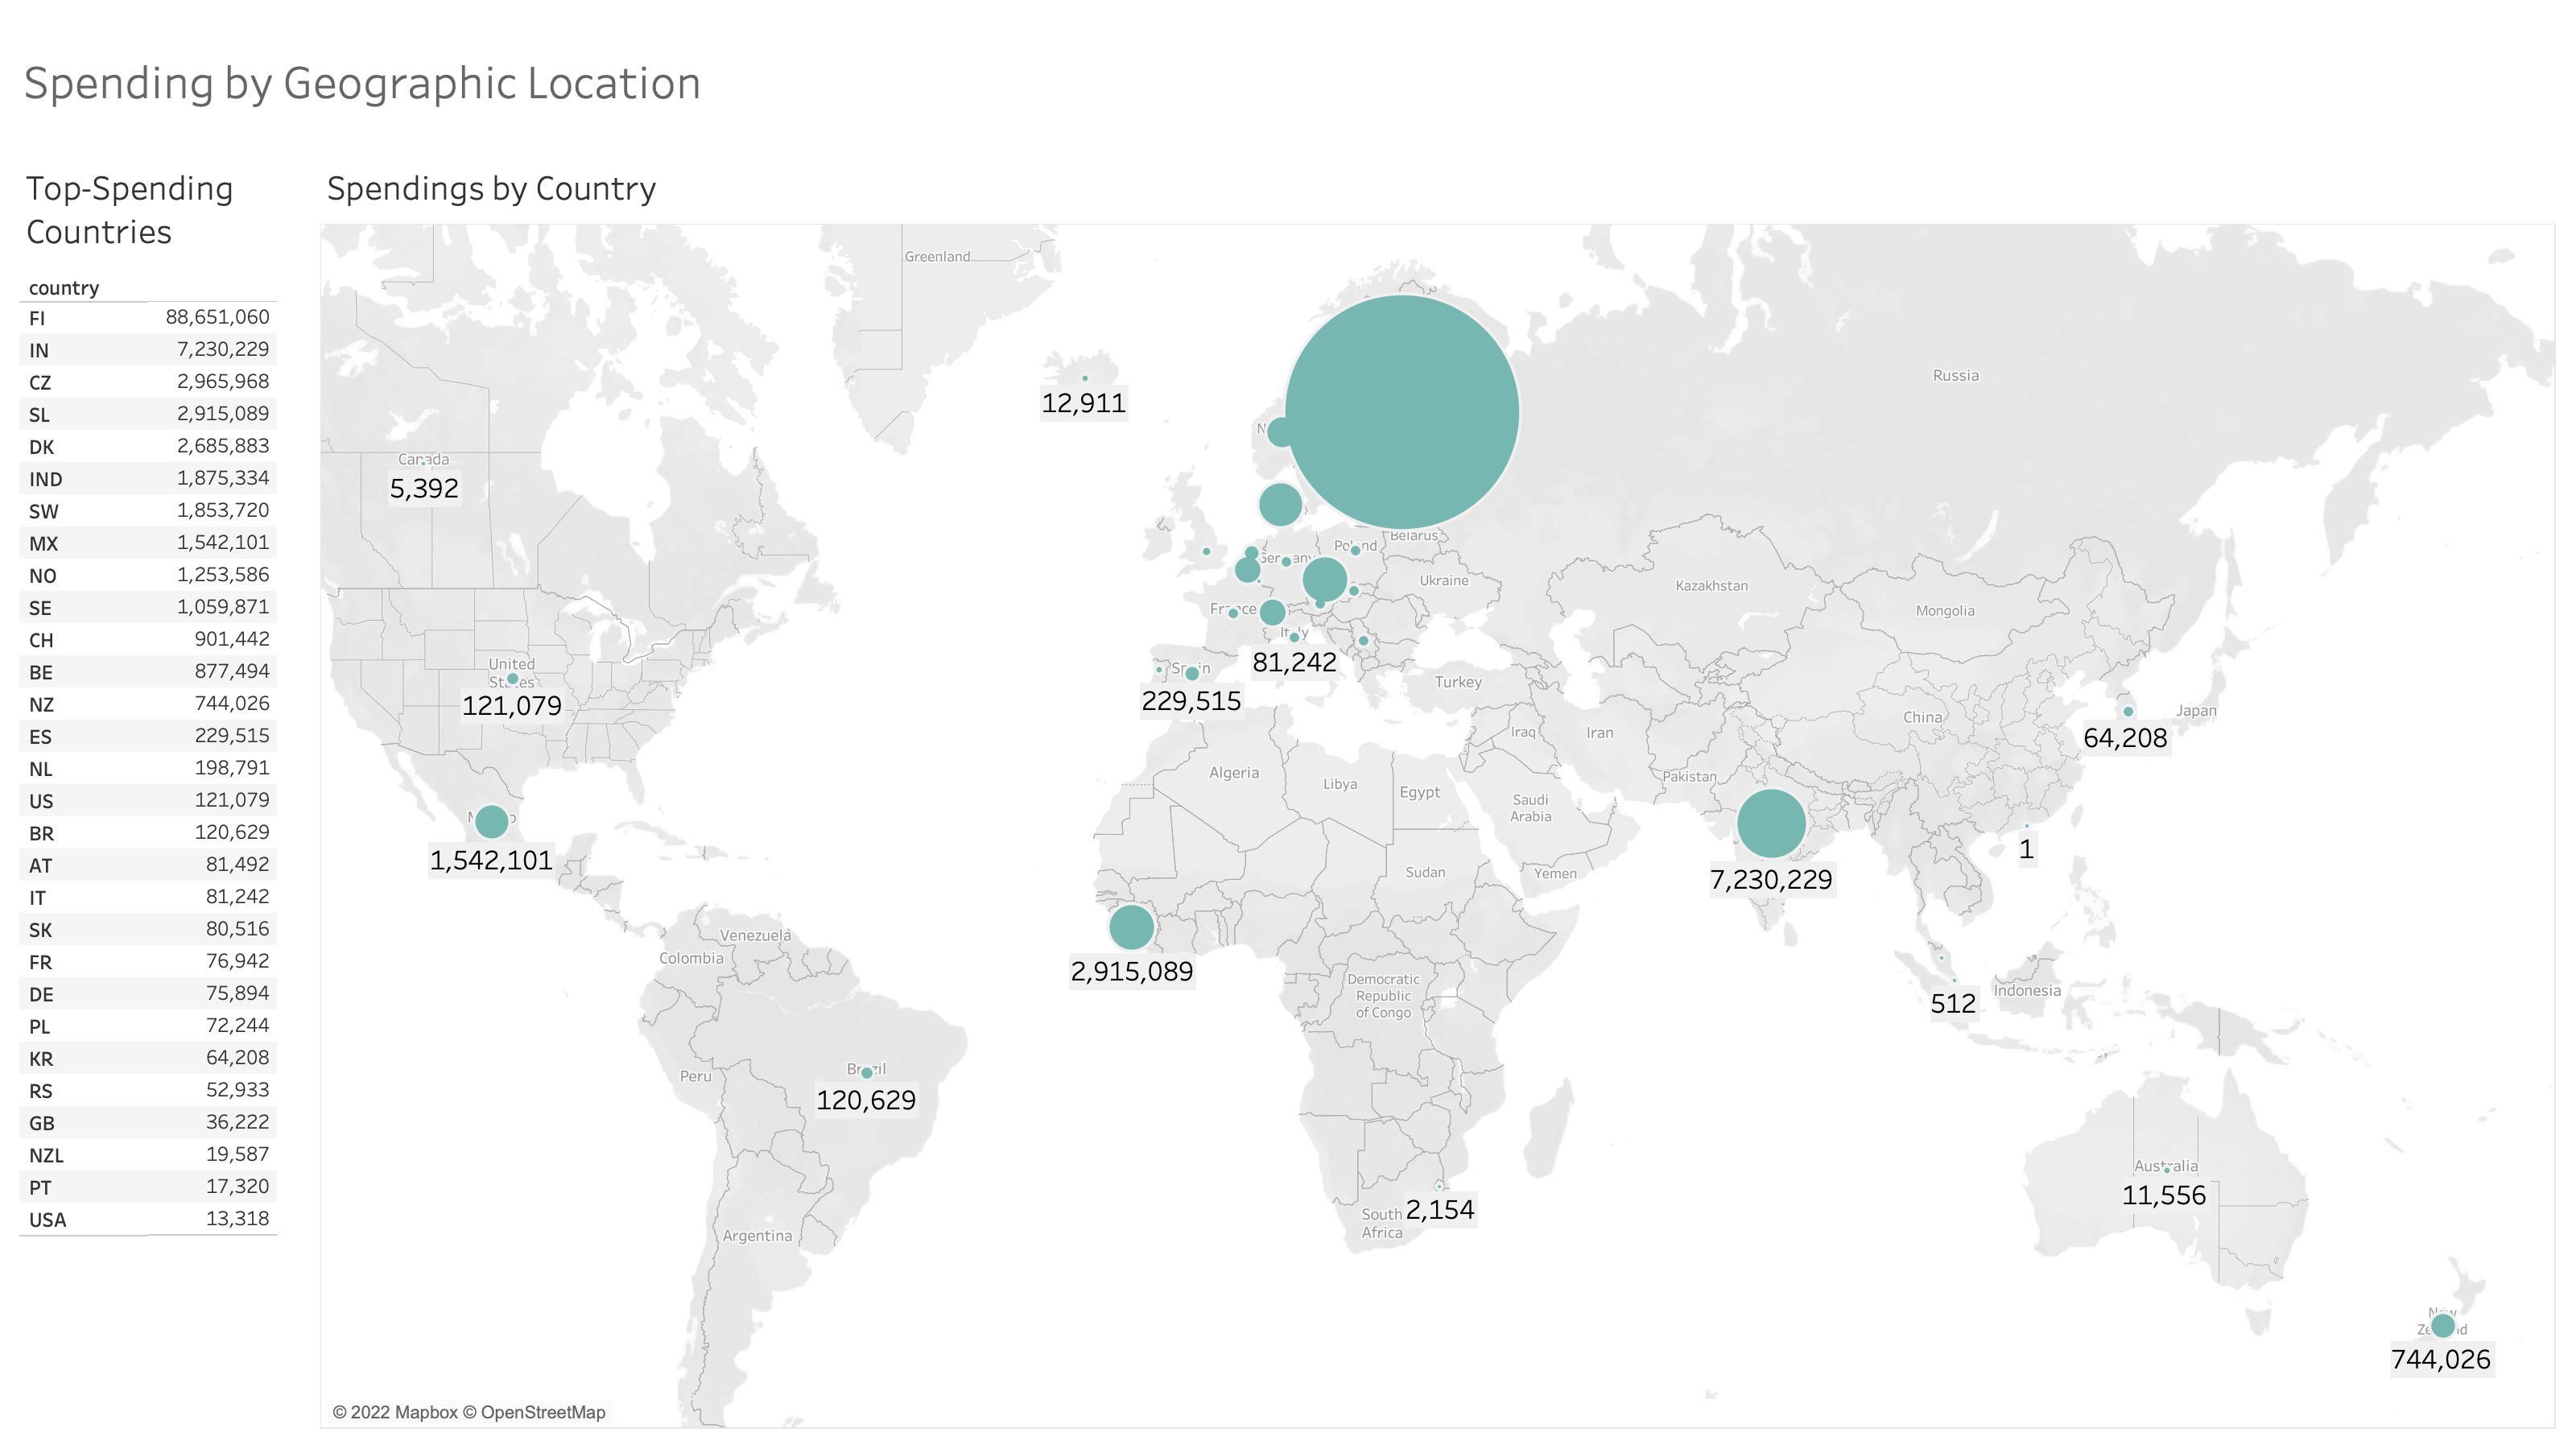
\includegraphics[width=\linewidth]{Bilder/deployment/world.png}
	\caption{Tableau Dashboard: Geographical Overview}
	\label{fig:dashboard-world}
\end{sidewaysfigure}

	The dashboard in Figure \ref{fig:dashboard-bubble} answers the questions 1-4. First, it shows the big picture of spending. Additional insights are in the tool tips of each bubble in the chart. The table on the left hand side provides a convenient overview of the different spending categories.
	
	The second dashboard in Figure \ref{fig:dashboard-world} concerns the questions 5 and 6. The map provides a quick insight into the impact of different company locations on spending. The information is shown with higher precision in the table on the left, which also gives a ranking of locations by expenses.
